\chapter{Robot Vision I: Image Processing}



% \todo[inline]{Edit blob\_search to add more guide comments}
% \todo[inline]{Do we need more HSV guidance?}
% \todo[inline]{Change showmask?}
% \todo[inline]{Make sure we mention circle/keypoints in blob search text}
\section{Important}
Read the entire lab before starting and especially the ``Grading" section so you are aware of all due dates and requirements associated with the lab.  There will be only one online session for this lab, so it is important that you prepare for that one opportunity to work with your TA.

\section{Scope}
\begin{itemize}
    \item Image Representation including Gray-scale image representation, Thresholding and Binarization.
    \item Image Processing including Filtering, Connectivity and Edge detection
    \item Image Analysis including Object segmentation, Pose estimation and Classification
\end{itemize}    

\section{Objectives}

This is the capstone lab of the semester and will integrate your work done in previous labs with python, ROS, and forward and inverse kinematics.  It will also introduce you to some basic OpenCV techniques.  In this lab you will:
\begin{itemize}
	\item Use OpenCV functions to distinguish the shape of the blocks and find the centroid and angle of them.
	\item Develop transformation equations that relate pixels in the image to coordinates in the world frame
	\item Report the world frame coordinates $(x_w,y_w)$ of the centroid of each block in the camera’s view.
	\item Move the block to a predefined position in the robot's work area.
\end{itemize}


\section{Background}

\begin{itemize}
	% \item Appendix \ref{computervision} which explains how to derive the intrinsic and extrinsic equations for the camera.
    % \item HSV Color Space:
    % \begin{itemize}
    % \item \url{https://en.wikipedia.org/wiki/HSL_and_HSV}
    % \item \href{https://stackoverflow.com/questions/10948589/choosing-the-correct-upper-and-lower-hsv-boundaries-for-color-detection-withcv}{https://stackoverflow.com/questions/10948589/}
    % \item \href{https://www.rapidtables.com/convert/color/rgb-to-hsv.html}{Converting RGB to HSV}
    % \end{itemize}
    
    % \item Simple Blob detector:
    % \begin{itemize}
    % \item \url{www.learnopencv.com/blob-detection-using-opencv-python-c/}
    % \item \href{https://stackoverflow.com/questions/8076889/how-to-use-opencv-simpleblobdetector}{https://stackoverflow.com/questions/8076889/}
    % \item \url{https://www.programcreek.com/python/example/89350/cv2.SimpleBlobDetector}
    % \item \url{https://www.programcreek.com/python/example/71388/cv2.SimpleBlobDetector_Params}
    % \end{itemize}
    \item Image Acquisition \\
Image sensors, like many other types of sensors, acquire signal from the surrounding to
obtain information pertaining to the environment. Signals can be generated from light wave,
or other form of energy for example (acoustic in ultrasound imaging) by an imaging system.
The process of acquiring images of the surrounding scene is an important aspect for robot
applications. As robots are usually expected to accomplish specific tasks while interacting with
the environment, a typical robot vision system involves processing video stream on-the-fly
for timely feedback control or decision making. Hence, connecting imaging systems to the
robot becomes an important aspect for robot vision.

A camera device is often used to acquire timely visual information of the surrounding. In
this lab, we will connect a camera to capture images represented as digital information for
processing and computational operation.
\end{itemize}



\begin{itemize}
    \item Image Processing \\
Behind the scenes of robot vision lies image processing operations that enhance, analyze
and/or transform the image data. In robot vision, a robot makes sense of the surrounding
through acquired and processed images that present useful information including colors,
geometries, structures and motions.

In this lab, we process images by applying thresholding, binarization and filtering. Image
analysis is performed through edge detection, object segmentation, pose estimation and
similarity score measurement.
\end{itemize}   


\section{Tasks}
In this lab, we will be using some built in functions in the \textbf{OpenCV} library to locate blocks based on their shape and find their centroids.  \textbf{OpenCV} is a powerful set of open source tools that are useful for computer vision tasks.  They will allow us to efficiently complete tasks without having to develop the algorithms ourselves.

% \subsection{Description}
In this lab, we have several randomly placed blocks with different shapes and directions under an industrial camera, as is showed in the \figref{lab5description}.
All we need to do is to stack the block of the \textbf{same shape} in the \textbf{same direction} together.
The destination is not specified. Any place in the upper right area is fine. 

\begin{figure}
	\centering
		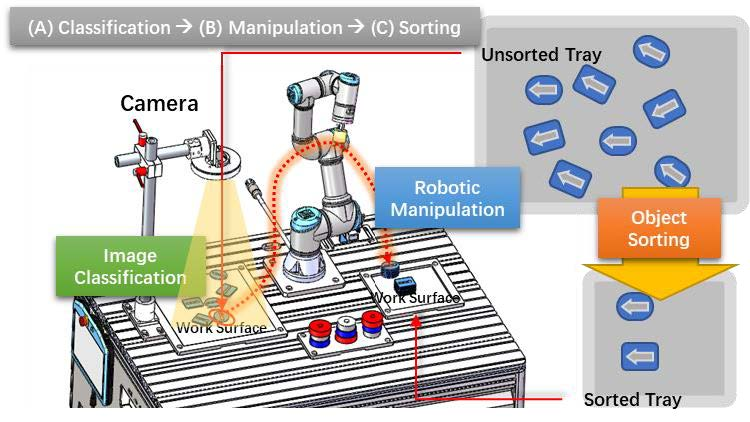
\includegraphics[scale=0.9]{image/lab6_table.jpg}
	\caption{\figlbl{lab5work} Task Description including Image Classification, Robot Manipulation and Object Sorting}
\end{figure}

\begin{figure}
	\centering
		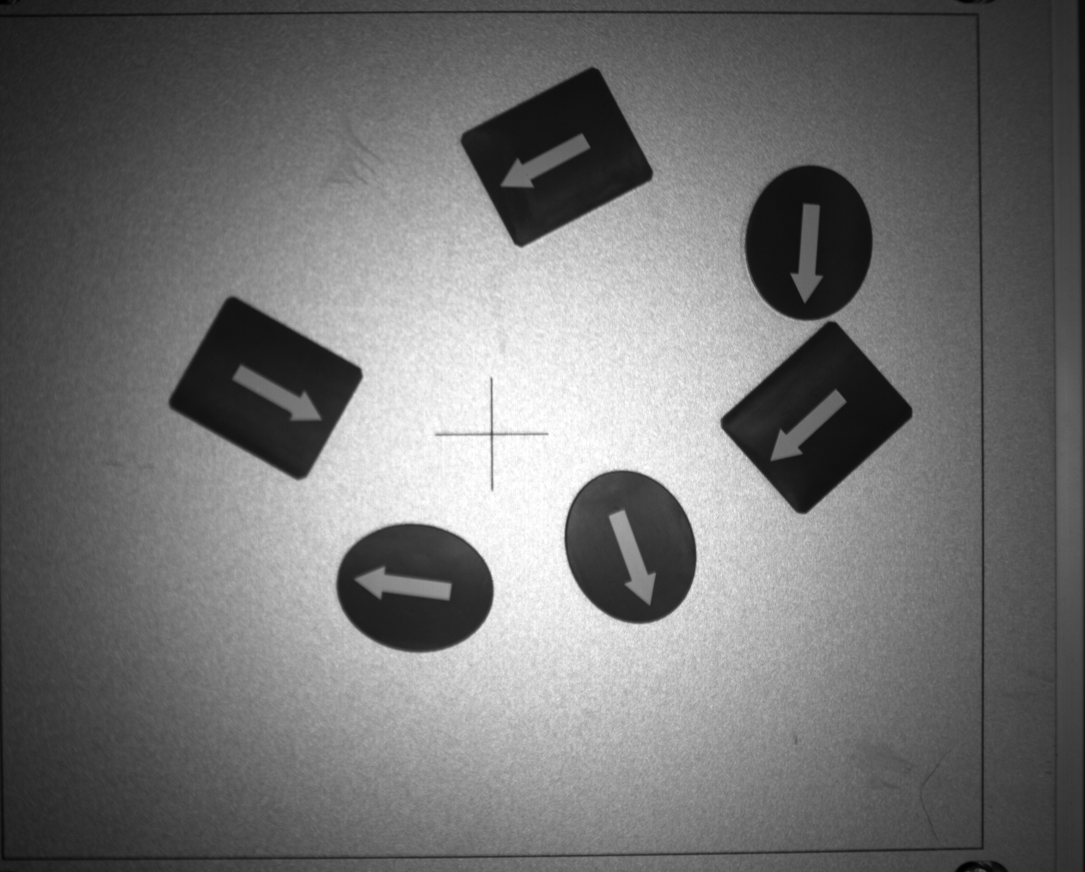
\includegraphics[scale=0.2]{image/lab6_real_pic.jpg}
	\caption{\figlbl{lab5description} Example of randomly placed blocks}
\end{figure}

\begin{figure}
	\centering
		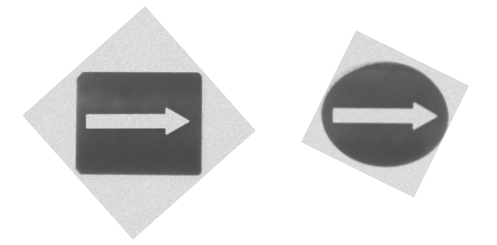
\includegraphics[scale=0.5]{image/lab6_example.jpg}
	\caption{\figlbl{lab5example} example.jpg}
\end{figure}

% Thresholding is the way we will isolate the objects that we are interested in by color.  We will be using the HSV color space to accomplish this.  HSV stands for Hue, Saturation and Value.  Using \textbf{OpenCV}, we will mask out any objects that don't fall within the desired HSV range that we set.  This allows us to focus only on the green and yellow blocks that we wish to locate.


% \textbf{Side Note:}  What is the H,S,V color space?  Please see the reference link to the Wikipedia  page discussing color spaces.  You are probably most familiar with the R,G,B (red,green,blue) color space.  Here each pixel of an image has a R,G,B value.  With H,S,V colors are placed on a color wheel and you indicate which color you are interested in by selecting an angle range.  In \textbf{OpenCV} the range of the angle is from 0 degrees to 180 degrees.  (You will find other implementations that use 0-360).  For example a blueish color would be in the angle range of 110 degrees to 130 degrees.  The S value is a number between 0 and 255 with 0 being very white and washed out and 255 the full, clear color.  The V value is also a number between 0 and 255 with 0 being very dark and shaded and 255 the full clear color.  The main reason we use the H,S,V color space in this lab is that it makes finding a color with different shading and lighting conditions much easier. 

% Once we have thresholded the image, we are left with `blobs'.  Blobs consist of the groups of pixels that were not masked out by thresholding.  No matter how well we perform thresholding, there will always be noise in the image.  We only really care about the blobs that correspond to the blocks we wish to find and the \textbf{OpenCV} function \textbf{SimpleBlobDectector} can help us do that.  It allows us to filter out blobs based on features like size, roundness, eccentricity, etc.  In addition, once we have narrowed down to the blobs we care about, it can help us find the centroid of these blobs.


% \subsection{Camera Calibration and Transformation}
% The problem of camera setup is that of relating (row,column) coordinates in an image to the corresponding coordinates in the world frame $(x_w,y_w,z_w)$.  A camera transformation equation will be developed to allow us to perform this conversion. Several parameters must be specified in order to implement the equations. Specifically, we are interested in \textbf{$\theta$} the rotation between the world frame and the camera frame and \textbf{$\beta$} the scaling constant between distances in the world frame and distances in the image and $T_{x}$ and $T_{y}$ the relationship between the origin of the camera frame and the world frame. Due to simulation limitations, these values and others have been provided for you.

% Appendix \ref{computervision} will guide you through the development of the camera transformation equations and explain the camera calibration process.

% \subsection{Pick and Place}
% Your program should:

% \begin{itemize}
% \item Move the Robot out of the way so that the camera can view the entire work area in order to find the blocks randomly placed in that area.  

% \item Use \textbf{OpenCV} functions to find the centroid $(x_w,y_w)$ of each block.

% \item Display a center point and a circle around each discovered block in the video display window.  

% \item Command the robot to pick up each block one at a time and place it in the appropriate goal position. 

% \item When finished with all blocks exit from the program.  

% \end{itemize}

\section{Procedure}
\subsection{Lab Set Up}
Start as you normally do by downloading the Lab 5 starter files from the lab website, unzip them and place them in your \textbf{src} directory along with the rest of the lab packages.

If you look inside \textbf{lab5pkg\_py/scripts}, you will see a number of Python files, but we will only be editing a few during this lab.  A brief description of each file is provided here:
\begin{itemize}
    \item \textbf{lab5\_exec.py} - The main executable.  It contains all the code to move the arm.  You will edit this to complete the pick and place task.
    % \item \textbf{lab5\_blob\_search.py} - This contains all the code related to image thresholding and finding blobs and centroids.  You will edit this to locate the desired objects and return their positions in pixel coordinates.
    % \item \textbf{lab5\_coordinate\_converter.py} - This contains the camera calibration and transformation code. You will edit this to add in the camera transformation equations.
    \item \textbf{lab5\_func.py} - This contains the forward and inverse kinematics code.  You should edit to add your solutions from Lab 3 and 4.
    \item \textbf{lab5\_header.py} - This is a standard header file with imports and constant definitions.  There is no need to edit this.
    % \item \textbf{lab5\_gen\_image.py} and \textbf{lab5\_spawn\_block.py} - These are used to generate blocks to pick up.  Do not edit.
    \item \textbf{lab5\_img.py} - This contains all the image processing, camera calibration and transformation code. You will edit this to process your image, find the camera transformation equation.
    \item \textbf{CMakeLists.txt} a file that sets up the necessary libraries and environment for compiling lab5\_exec.py.
    \item \textbf{package.xml} This file defines properties about the package including package dependencies.
    \item \textbf{README} To run lab5 code on real robot, please read it \textbf{FIRST}!
    \item Every time you open a new terminal, you need to run \textbf{source devel/setup.bash} in your catkin folder.
    
\end{itemize}

\subsection{Image Acquisition}
In this lab, we just capture the image manually. First, copy the folder \textbf{Snapshot} in folder \textbf{lab5pkg} to the \textbf{Windows} System.
Then you can edit the python script \textbf{save\_image.py} to change the directory where your snapshots will save
before you run it to store a series of images. After that, we can use these images in our ROS programming.

\subsection{Image Processing}

In order to distinguish the shape of the blocks, we use a template matching method here. 
The \textbf{example.jpg} ,shown in \figref{lab5example},is the given template, including a rectangular block and an elliptical one.
Then the similarity measurement of the target block can help with the classification problem when comparing with the template.

{\footnotesize
%\tiny{
%\begin{verbatim}[obeytabs,tabsize=4]
%\footnotesize{
\begin{verbatim}
    rospack = rospkg.RosPack()
    lab5_path = rospack.get_path('lab5pkg_py')
    img_path = os.path.join(lab5_path, 'scripts', 'example.jpg')
    _img = cv2.imread(img_path)
    _draw_img = _img.copy()

    _blur = cv2.bilateralFilter(_img, 19, 130, 30)
    _blur = cv2.medianBlur(_blur, 9)

    _img_gray = cv2.cvtColor(_blur, cv2.COLOR_BGR2GRAY)
    _xgrd = cv2.Sobel(_img_gray, cv2.CV_16SC1, 1, 0)
    _ygrd = cv2.Sobel(_img_gray, cv2.CV_16SC1, 0, 1)
    _img = cv2.Canny(_xgrd, _ygrd, 30, 220)
\end{verbatim}}
Code Explanation: First, we obtain the path to the template \textbf{example.jpg} and read it subsequently by the \textbf{OpenCV} method \textbf{cv2.imread}.
Then we preprocess the image by \textbf{cv2.bilateralFilter} and \textbf{cv2.medianBlur}.
Bilateral filter can smooth images while preserving edges by means of a nonlinear combination of nearby image values.
And median filter is also common to eliminate isolated noise.
After converting image to gray-scale using \textbf{cv2.cvtColor}, we can exploit \textbf{Sobel} and \textbf{Canny} operator
to detect the edge of the template.

\begin{figure}
	\centering
		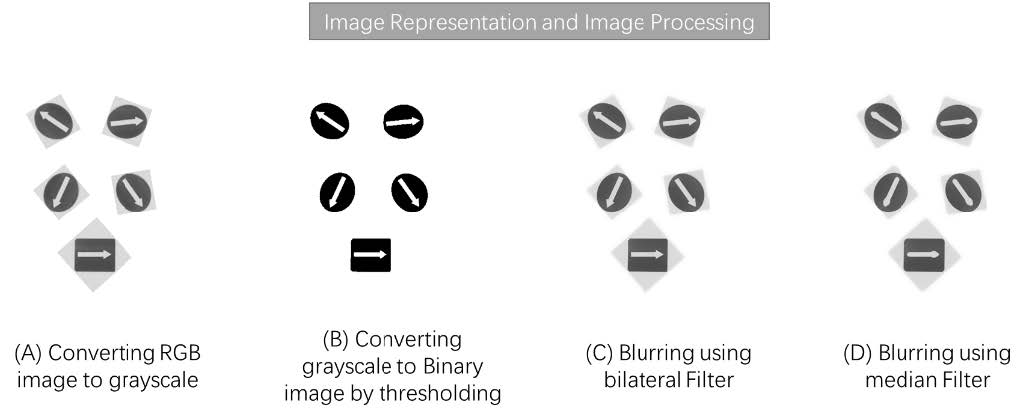
\includegraphics[scale=1]{image/lab6_img_process.jpg}
	\caption{\figlbl{lab5_1} Image Representation and Image Processing}
\end{figure}

\begin{figure}
	\centering
		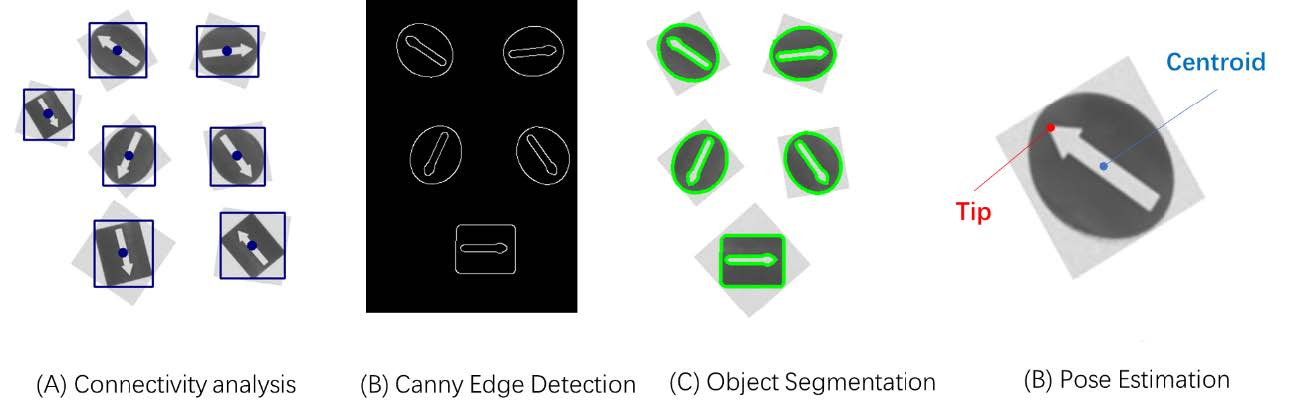
\includegraphics[scale=0.9]{image/lab6_edge.jpg}
	\caption{\figlbl{lab5_2} Image Representation and Image Processing}
\end{figure}

{\footnotesize
%\tiny{
%\begin{verbatim}[obeytabs,tabsize=4]
%\footnotesize{
\begin{verbatim}
    _w, _h = _img.shape
    # rectangle
    _img_1 = _img[:, :_w]
    # ellipse
    _img_2 = _img[:, _w:]

    # rectangle
    _img_1, _contours_1, hierarchy = cv2.findContours(_img_1, cv2.RETR_TREE, cv2.CHAIN_APPROX_SIMPLE)
    # ellipse
    _img_2, _contours_2, hierarchy = cv2.findContours(_img_2, cv2.RETR_TREE, cv2.CHAIN_APPROX_SIMPLE)
\end{verbatim}}

Code Explanation: Here we divide the image into two parts, i.e., rectangle and ellipse.
Then we use \textbf{cv2.findContours} to find contours. Variables \textbf{\_contours\_1} and \textbf{\_contours\_2} store all contours, each of which is composed of
a series of pixel points.\\
\textbf{IMPORTANT}: Before you use the contours found by \textbf{cv2.findContours}, please check and ensure these are what you want!
And Try to figure out why the number of contours is twice.

{\footnotesize
%\tiny{
%\begin{verbatim}[obeytabs,tabsize=4]
%\footnotesize{
\begin{verbatim}
    # compute the center of a contour
    N = cv2.moments(contours[i * 2])
    _center_x = int(N["m10"] / N["m00"])
    _center_y = int(N["m01"] / N["m00"])
    # draw a circle on the center point
    cv2.circle(draw_img, (int(_center_x), int(_center_y)), 7, [0,255,0], -1)
\end{verbatim}}

Code Explanation: Here we use \textbf{cv2.moments} to compute the centroids and label a circle on the center point
by \textbf{cv2.circle}.


% \subsection{Running the Program}
% To run the code, open a terminal window and in your catkin working directory:
	
% % \begin{lstlisting}[language=bash]
% %     $ source devel/setup.bash
% %     $ roslaunch lab5pkg_py lab5.launch
% % \end{lstlisting}
% \begin{lstlisting}[language=bash]
%     $ source devel/setup.bash
%     $ roslaunch ur3_driver ur3_gazebo.launch
% \end{lstlisting}

% Then open a second terminal window and in your catkin working directory:
    
% \begin{lstlisting}[language=bash]
%     $ source devel/setup.bash
%     $ rosrun lab5pkg_py lab5_coordinate_converter.py
% \end{lstlisting}

% Then open a third terminal window and in your catkin working directory:
    
% \begin{lstlisting}[language=bash]
%     $ source devel/setup.bash
%     $ rosrun lab5pkg_py lab5_exec.py --missing False 
%     --image 0
% \end{lstlisting}


% The -{}-\textit{missing} flag, when \textbf{True}, will allow you to test your gripper feedback implementation.  The -{}-\textit{image} flag will change what image is being displayed.  It is normally set to image 0, but can be changed so you can test all 5 images i.e 0 to 4.  Each image represents a different set of block locations.  Your final code must work on all five images. The code has been divided up like this to aid you in working with it.  You should not need to restart Gazebo while making edits to files, but you can easily restart the coordinate converter node after you edit that file.  The executable will naturally stop after completing its tasks.

% When you run the program, you will see two image windows pop-up.  One is the color or raw image.  The other is a black and while masked image that will change based on your threshold values.  Note that sometimes the two windows will appear on top of each other making it appear that one is not present.  Simply move the top window to see both.



% \subsection{Threshold camera image to distinguish the colors of choice} \label{ObjCentriod}
% In \textbf{lab5\_blob\_search.py}, in the function \textbf{blob\_search(...)}, you will edit the following to locate the green and yellow blocks.  They are currently set to threshold blue colored objects.
% {\footnotesize
% \begin{verbatim}
%     lower = (110, 50, 50)   # Blue lower
%     upper = (130, 255, 255) # Blue upper
% \end{verbatim}}

% Selecting the correct values for thresholding can be rather challenging and requires some trial and error.  There are several methods that you can use to find these values.  One is to review how the HSV color space works and select an appropriate Hue value.  Once that is selected, you should adjust Saturation and Value until a clean image is created.  If necessary, you may need to widen or narrow your Hue range.  Another method is to convert the RGB value given in the image window to an HSV value.  Note the RGB values displayed in the lower left hand corner of \figref{centroid}.  They represent the RGB value of what ever pixel the mouse pointer is hovering over.  Using these values in a website like the one listed in the references will allow you to get a starting point for your HSV ranges.  Pay attention to how the HSV value is represented on the website compared to the way it is represented in \textbf{OpenCV}. Note that you will have to create a different set of ranges for for each color and select the appropriate range depending on what color you are looking for.

% When successfully completed, you will see a black and white image with white shaped blobs that have little `noise' inside their boundaries.  It is okay to have more than one blob in the image as long the block we desire is seen as this process works in conjunction with blob detection to isolate the desired block.  See \figref{thresh} for reference. You will only see one threshold image at a time.  When you you are done viewing the image, you should press the enter key to move to the next step - make sure the image window is selected when you hit enter and not a terminal or other window.
% \begin{figure}[ht]
% \centering
% 	
\includegraphics[height=6cm]{lab5_threshold.png}
% \caption{\figlbl{thresh} A well thresholded image.  Note you can see the block clearly.}
% \end{figure}


% \subsection{Blob Detection}
% In \textbf{lab5\_blob\_search.py}, in the function \textbf{blob\_search(...)}, you will edit the following to identify blobs within the thresholded image.
% {\footnotesize
% \begin{verbatim}
%     # Setup SimpleBlobDetector parameters.
%     params = cv2.SimpleBlobDetector_Params()

%     # Filter by Color
%     params.filterByColor = False

%     # Filter by Area.
%     params.filterByArea = False

%     # Filter by Circularity
%     params.filterByCircularity = False

%     # Filter by Inertia
%     params.filterByInertia = False

%     # Filter by Convexity
%     params.filterByConvexity = False
% \end{verbatim}}
% Currently all the `filterBy...' parameters are set to False.  You need to decide which filter parameters you want to use to limit the detected blobs to the block you care about.  This is done by setting it to \textbf{True} and adding the necessary parameters to the code.  You should consult the \textbf{OpenCV} references for help in understanding what these parameters mean and how to properly set them.  It is not necessary or desirable to use all the parameters, so you only need to select the ones that you think will help. When set correctly, the only keypoints detected will be those of the desired block and their centroids will be drawn accurately on the block as seen in \figref{centroid}. Note that these parameters will have no effect on the mask view, only the keypoints found.  In order to mark the keypoints and draw a circle around the block, complete the following code and uncomment them:
% {\footnotesize
% \begin{verbatim}
%     # Draw a circle around the detected block
%     # im_with_keypoints = cv2.circle(image_raw, (int(c), int(r)), ???)

%     # Draw the keypoints on the detected block
%     # im_with_keypoints = cv2.drawKeypoints(im_with_keypoints, keypoints, ???)


% \end{verbatim}}

% \begin{figure}[ht]
% \centering
% 	
\includegraphics[height=6cm]{lab5_centroid.png}
% \caption{\figlbl{centroid} A properly drawn centroid on the block.}
% \end{figure}



% \subsubsection{Camera Calibration}
% Camera calibration is the process of figuring out the parameters used in the camera transformation. \textbf{lab5\_coordinate\_converter.py} contains these values.
% {\footnotesize
% \begin{verbatim}
%     # Params for camera calibration
%     theta = -0.09
%     beta = 730.0
%     tx = -0.297435628054
%     ty = -0.0763807206584
% \end{verbatim}}


% \subsubsection{Camera Transformation}
% Camera transformation will be completed in in \textbf{lab5\_coordinate\_converter.py}.  You should work through the process of finding the camera transformation equations in Appendix \ref{computervision}.  These equations will then be entered into the function \textbf{IMG2W(r,c)}.  The goal of this function is to take the received pixel values and convert them to world frame coordinates in meters.  When you update this file, you need to restart the coordinate converter node for the changes to take effect.

% \subsection{Pick and Place}
% To complete the pick and place portion of this lab, you will need to edit \textbf{lab5\_exec.py}.  There are a number of tasks in this section that should be familiar to you from Lab 2.  
% In the \textbf{main()} function, you will have to complete the logic of the pick and place task. 


% {\footnotesize
% \begin{verbatim}
%     # Call blob search
%     green_image_rc = blob_search(cv_image.copy(), 'green')
%     yellow_image_rc = blob_search(cv_image.copy(), 'yellow')
% \end{verbatim}}

% After calling \textbf{blob\_search(...)}, you will have the location of the green and yellow blocks in pixels.  You will then need to pass this data to \textbf{lab5\_coordinate\_converter.py} so we can get the position in world coordinates.  To do this, we will create a publisher to pass the pixel values to our coordinate converter.  Then, when it is done converting the image, we will subscribe to the coordinate converter's output.  Note that a small break between the publishing the data to the image coordinate converter and making use of the subscriber's output maybe needed to prevent accessing old data (Suggestion: Look at \textbf{rospy.sleep(...)}).  The publisher and subscriber will use the \textbf{Point} message type and you should research this to figure out what data it contains.

% You will also need to complete the \textbf{move\_block(...)} function.  While this is similar to the work done in Lab 2, we now no longer have hard coded angle values.  You will need to use your inverse kinematics to find these angles.  The goal positions are provided in the code.  Additionally, your \textbf{move\_block(...)} function should detect missing blocks as you did in Lab 2.  If a missing block is found the program should move the arm back to home and halt the program with an error message.

% When complete, you will be able to run the code on any of the five images and it will locate, pick up and place both colored blocks.

\subsection{Debugging}
This lab can be a bit tricky to work through as several parts require trial and error.  Here are some suggestions:
\begin{itemize}
    \item Approach the lab sequentially and make sure you get good results at each step.
    \item Comment out parts that you are not currently using (Don't forget the uncomment them though...)
\end{itemize}


\section{Report}
This lab does not require a formal lab report - only the submission of your code.  You should a submit a document to \href{https://learn.intl.zju.edu.cn/}{Blackboard} containing all of the files that you edited to complete the lab.  This will be submitted to \href{https://learn.intl.zju.edu.cn/}{Blackboard} as in the past.

\section{Demo}
Your TA will require you to run your program twice, each time with different initial block positions and verify that your program can locate the blocks and place them in the correct location.  You will also demonstrate that suction feedback is working.

\section{Grading}
\begin{itemize}
\item 100 points, successful demonstration and submission of the code. (No code = 0 points)
\end{itemize}


% \section{Tentative Due Dates - Fall 2020}
% Lab 5 demonstration will be due by 5PM on Wednesday, December 16.  Code must be submitted on \href{www.gradescope.com}{GradeScope}, by midnight that same day.  Note that each TA will only have a limited number of office hours prior to this time, so you should plan ahead to meet this deadline.
